\documentclass{standalone}
\usepackage{tikz}
\usetikzlibrary{calc,intersections}
\begin{document}
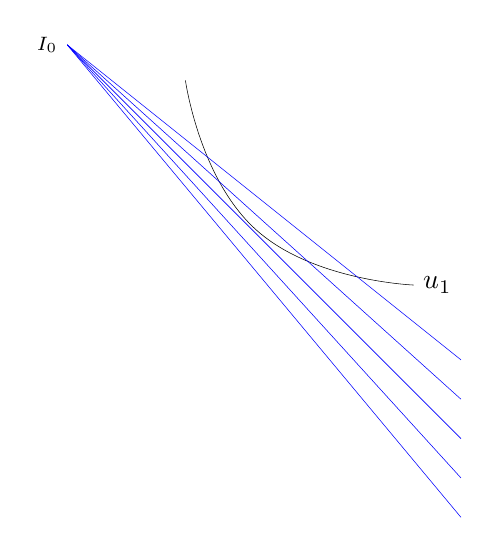
\begin{tikzpicture}
    % u_1
    \node (h) at (1.5,4.2) {};
    \node (b) at (2.4,2.3) {};
    \node (j) at (4.4,1.6) {};
    \draw[very thin,name path=curve 1] plot[smooth,tension=0.9] 
          coordinates {(h) (b) (j)} node[right]{$u_{1}$};
    \coordinate[label=left:{\scriptsize$I_{0}$}] (i0) at (0,4.65);
 \foreach \p in {-1.2,-1.1,...,-0.8}
 {\draw[blue,very thin] (0,4.65) -- (5,5*\p+4.65);}    
\end{tikzpicture}
\end{document}